\documentclass[a4paper]{book}
\usepackage{a4wide}
\usepackage{makeidx}
\usepackage{graphicx}
\usepackage{multicol}
\usepackage{float}
\usepackage{listings}
\usepackage{color}
\usepackage{textcomp}
\usepackage{alltt}
\usepackage{times}
\usepackage{ifpdf}
\ifpdf
\usepackage[pdftex,
            pagebackref=true,
            colorlinks=true,
            linkcolor=blue,
            unicode
           ]{hyperref}
\else
\usepackage[ps2pdf,
            pagebackref=true,
            colorlinks=true,
            linkcolor=blue,
            unicode
           ]{hyperref}
\usepackage{pspicture}
\fi
\usepackage[utf8]{inputenc}
\usepackage{doxygen}
\lstset{language=C++,inputencoding=utf8,basicstyle=\footnotesize,breaklines=true,breakatwhitespace=true,tabsize=8,numbers=left }
\makeindex
\setcounter{tocdepth}{3}
\renewcommand{\footrulewidth}{0.4pt}
\begin{document}
\hypersetup{pageanchor=false}
\begin{titlepage}
\vspace*{7cm}
\begin{center}
{\Large Aibo Player Driver }\\
\vspace*{1cm}
{\large Generated by Doxygen 1.6.1}\\
\vspace*{0.5cm}
{\small Fri Apr 16 11:04:01 2010}\\
\end{center}
\end{titlepage}
\clearemptydoublepage
\pagenumbering{roman}
\tableofcontents
\clearemptydoublepage
\pagenumbering{arabic}
\hypersetup{pageanchor=true}
\chapter{Class Index}
\section{Class Hierarchy}
This inheritance list is sorted roughly, but not completely, alphabetically:\begin{DoxyCompactList}
\item \contentsline{section}{AiboCore}{\pageref{classAiboCore}}{}
\item \contentsline{section}{AiboHead}{\pageref{classAiboHead}}{}
\item \contentsline{section}{AiboNet}{\pageref{classAiboNet}}{}
\item \contentsline{section}{AiboWalk}{\pageref{classAiboWalk}}{}
\item \contentsline{section}{dev}{\pageref{classdev}}{}
\begin{DoxyCompactList}
\item \contentsline{section}{AiboCam}{\pageref{classAiboCam}}{}
\end{DoxyCompactList}
\end{DoxyCompactList}

\chapter{Class Index}
\section{Class List}
Here are the classes, structs, unions and interfaces with brief descriptions:\begin{DoxyCompactList}
\item\contentsline{section}{\hyperlink{classAiboCam}{AiboCam} (Aibo's Camera This class represents and implements methods to capture images from the Aibo. Image details are initialized here: depth = 3 -\/ Does not change width = 0 -\/ Automatically resized when initialized() called height = 0 -\/ Automatically rezied when inttialized() called )}{\pageref{classAiboCam}}{}
\item\contentsline{section}{\hyperlink{classAiboCore}{AiboCore} (The entire Aibo and required Player classes. Core of driver )}{\pageref{classAiboCore}}{}
\item\contentsline{section}{\hyperlink{classAiboHead}{AiboHead} (Controls the Aibo's head. The \hyperlink{classAiboHead_adf0f91fafeaa5e32b5e387ac136e0f37}{move()} function is designed to work with the parameters provided by the PTZ Player interface )}{\pageref{classAiboHead}}{}
\item\contentsline{section}{\hyperlink{classAiboNet}{AiboNet} (Class responsible for low level network communications )}{\pageref{classAiboNet}}{}
\item\contentsline{section}{\hyperlink{classAiboWalk}{AiboWalk} (Control's the Aibo's movement (Walking). The \hyperlink{classAiboWalk_ace69bca076d0091769b1af5ca7636953}{walk()} function is designed to be used with the parameters provided by the Position2d interface )}{\pageref{classAiboWalk}}{}
\item\contentsline{section}{\hyperlink{classdev}{dev} (This class just wraps the image used by \hyperlink{classAiboCam}{AiboCam} )}{\pageref{classdev}}{}
\end{DoxyCompactList}

\chapter{Class Documentation}
\hypertarget{classAiboCam}{
\section{AiboCam Class Reference}
\label{classAiboCam}\index{AiboCam@{AiboCam}}
}


Aibo's Camera This class represents and implements methods to capture images from the Aibo. Image details are initialized here: depth = 3 -\/ Does not change width = 0 -\/ Automatically resized when initialized() called height = 0 -\/ Automatically rezied when inttialized() called.  


{\ttfamily \#include $<$AiboCam.h$>$}Inheritance diagram for AiboCam:\nopagebreak
\begin{figure}[H]
\begin{center}
\leavevmode
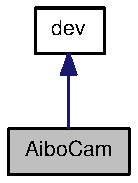
\includegraphics[width=102pt]{classAiboCam__inherit__graph}
\end{center}
\end{figure}
Collaboration diagram for AiboCam:\nopagebreak
\begin{figure}[H]
\begin{center}
\leavevmode
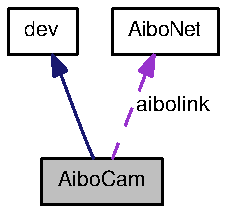
\includegraphics[width=144pt]{classAiboCam__coll__graph}
\end{center}
\end{figure}
\subsection*{Public Member Functions}
\begin{DoxyCompactItemize}
\item 
\hypertarget{classAiboCam_a594411a1df57552aa2b9c609319c74d4}{
\hyperlink{classAiboCam_a594411a1df57552aa2b9c609319c74d4}{AiboCam} ()}
\label{classAiboCam_a594411a1df57552aa2b9c609319c74d4}

\begin{DoxyCompactList}\small\item\em Aibo's Camera This class represents and implements methods to capture images from the Aibo. Image details are initialized here: depth = 3 -\/ Does not change width = 0 -\/ Automatically resized when initialized() called height = 0 -\/ Automatically rezied when inttialized() called. \item\end{DoxyCompactList}\item 
int \hyperlink{classAiboCam_a72162af9d25b9b24d6449d41b234f8b2}{updateMMap} (int decompress)
\item 
void \hyperlink{classAiboCam_aa450f46c7d0bfc09ec6f6b16cb42fdc6}{connect} (const char $\ast$ip\_\-addr)
\item 
\hyperlink{classAiboCam_aeef7ebf6fe97788c0672481399586295}{$\sim$AiboCam} ()
\end{DoxyCompactItemize}


\subsection{Detailed Description}
Aibo's Camera This class represents and implements methods to capture images from the Aibo. Image details are initialized here: depth = 3 -\/ Does not change width = 0 -\/ Automatically resized when initialized() called height = 0 -\/ Automatically rezied when inttialized() called. 

\subsection{Constructor \& Destructor Documentation}
\hypertarget{classAiboCam_aeef7ebf6fe97788c0672481399586295}{
\index{AiboCam@{AiboCam}!$\sim$AiboCam@{$\sim$AiboCam}}
\index{$\sim$AiboCam@{$\sim$AiboCam}!AiboCam@{AiboCam}}
\subsubsection[{$\sim$AiboCam}]{\setlength{\rightskip}{0pt plus 5cm}AiboCam::$\sim$AiboCam ()}}
\label{classAiboCam_aeef7ebf6fe97788c0672481399586295}
RWLock used to prevent RWLock lock; /$\ast$! Deconstructor for \hyperlink{classAiboCam}{AiboCam}. Deletes aibolink (socket)

Deconstructor for \hyperlink{classAiboCam}{AiboCam}. Deletes aibolink (socket) 

\subsection{Member Function Documentation}
\hypertarget{classAiboCam_aa450f46c7d0bfc09ec6f6b16cb42fdc6}{
\index{AiboCam@{AiboCam}!connect@{connect}}
\index{connect@{connect}!AiboCam@{AiboCam}}
\subsubsection[{connect}]{\setlength{\rightskip}{0pt plus 5cm}void AiboCam::connect (const char $\ast$ {\em hostname})}}
\label{classAiboCam_aa450f46c7d0bfc09ec6f6b16cb42fdc6}
Creates and connects a socket to capture images from the Aibo 
\begin{DoxyParams}{Parameters}
\item[{\em $\ast$hostname}]-\/ Pointer to the ip address of the Aibo \end{DoxyParams}
\hypertarget{classAiboCam_a72162af9d25b9b24d6449d41b234f8b2}{
\index{AiboCam@{AiboCam}!updateMMap@{updateMMap}}
\index{updateMMap@{updateMMap}!AiboCam@{AiboCam}}
\subsubsection[{updateMMap}]{\setlength{\rightskip}{0pt plus 5cm}int AiboCam::updateMMap (int {\em decompress} = {\ttfamily 1})}}
\label{classAiboCam_a72162af9d25b9b24d6449d41b234f8b2}
Captures images from socket. Argument is used to toggle decompression of image. 
\begin{DoxyParams}{Parameters}
\item[{\em decompress}]-\/ jpeg decompression option 1 = decompress 0 = no-\/decompress \end{DoxyParams}


The documentation for this class was generated from the following files:\begin{DoxyCompactItemize}
\item 
/home/jesse/Dropbox/Aibo/src/AiboCam.h\item 
/home/jesse/Dropbox/Aibo/src/AiboCam.cc\end{DoxyCompactItemize}

\hypertarget{classAiboCore}{
\section{AiboCore Class Reference}
\label{classAiboCore}\index{AiboCore@{AiboCore}}
}


The entire Aibo and required Player classes. Core of driver.  


{\ttfamily \#include $<$AiboCore.h$>$}Collaboration diagram for AiboCore:\subsection*{Public Member Functions}
\begin{DoxyCompactItemize}
\item 
\hypertarget{classAiboCore_a673c057ac82df3fc6c0d828a98408bea}{
{\bfseries AiboCore} (const char $\ast$ip\_\-addr)}
\label{classAiboCore_a673c057ac82df3fc6c0d828a98408bea}

\item 
\hypertarget{classAiboCore_a377640056394d6235609688045288fe7}{
{\bfseries AiboCore} (ConfigFile $\ast$cf, int section)}
\label{classAiboCore_a377640056394d6235609688045288fe7}

\item 
\hypertarget{classAiboCore_a078c3b2541d57e7455094ef7c9e46c80}{
void {\bfseries connect} (const char $\ast$ip\_\-addr)}
\label{classAiboCore_a078c3b2541d57e7455094ef7c9e46c80}

\item 
\hypertarget{classAiboCore_a7cf6b6a288291b36254dc29ae089d6bc}{
int {\bfseries count} ()}
\label{classAiboCore_a7cf6b6a288291b36254dc29ae089d6bc}

\item 
\hypertarget{classAiboCore_a940aa3f41c521cfc8e1ea69b8a616648}{
virtual int {\bfseries MainSetup} ()}
\label{classAiboCore_a940aa3f41c521cfc8e1ea69b8a616648}

\item 
\hypertarget{classAiboCore_a4a06b4d7957998e00ffa662ff9345662}{
virtual void {\bfseries MainQuit} ()}
\label{classAiboCore_a4a06b4d7957998e00ffa662ff9345662}

\item 
\hypertarget{classAiboCore_a2612cdb01d22f3b18fa0c42ec15b4525}{
int {\bfseries ProcessMessage} (QueuePointer \&resp\_\-queue, player\_\-msghdr $\ast$hdr, void $\ast$data)}
\label{classAiboCore_a2612cdb01d22f3b18fa0c42ec15b4525}

\end{DoxyCompactItemize}
\subsection*{Public Attributes}
\begin{DoxyCompactItemize}
\item 
\hypertarget{classAiboCore_a0bfbdcab738086d571c8dd9936408221}{
\hyperlink{classAiboWalk}{AiboWalk} {\bfseries walk}}
\label{classAiboCore_a0bfbdcab738086d571c8dd9936408221}

\item 
\hypertarget{classAiboCore_a82f60f050d49dc500a23beff1c80d658}{
\hyperlink{classAiboHead}{AiboHead} {\bfseries head}}
\label{classAiboCore_a82f60f050d49dc500a23beff1c80d658}

\item 
\hypertarget{classAiboCore_ac299b12604a05d4be74eafac7162ba10}{
\hyperlink{classAiboCam}{AiboCam} {\bfseries cam}}
\label{classAiboCore_ac299b12604a05d4be74eafac7162ba10}

\end{DoxyCompactItemize}


\subsection{Detailed Description}
The entire Aibo and required Player classes. Core of driver. 

The documentation for this class was generated from the following files:\begin{DoxyCompactItemize}
\item 
/home/jesse/Dropbox/Aibo/src/AiboCore.h\item 
/home/jesse/Dropbox/Aibo/src/AiboCore.cc\end{DoxyCompactItemize}

\hypertarget{classAiboHead}{
\section{AiboHead Class Reference}
\label{classAiboHead}\index{AiboHead@{AiboHead}}
}


Controls the Aibo's head. The \hyperlink{classAiboHead_adf0f91fafeaa5e32b5e387ac136e0f37}{move()} function is designed to work with the parameters provided by the PTZ Player interface.  


{\ttfamily \#include $<$AiboHead.h$>$}Collaboration diagram for AiboHead:\nopagebreak
\begin{figure}[H]
\begin{center}
\leavevmode
\includegraphics[width=108pt]{classAiboHead__coll__graph}
\end{center}
\end{figure}
\subsection*{Public Member Functions}
\begin{DoxyCompactItemize}
\item 
void \hyperlink{classAiboHead_a5fef344c99e421b7c704099628ca3542}{connect} (const char $\ast$ip\_\-addr)
\item 
int \hyperlink{classAiboHead_a085f54c6374d5eb117c12b0e9cad2d0e}{up} (float magnitude)
\item 
int \hyperlink{classAiboHead_a60bd059ca7a58ee2b3ee95011150ea89}{down} (float magnitude)
\item 
int \hyperlink{classAiboHead_a4821a0ccff77b881636aec49703a3683}{left} (float magnitude)
\item 
int \hyperlink{classAiboHead_a6be7b6743be53896c2f41dc1db1ce2a5}{right} (float magnitude)
\item 
int \hyperlink{classAiboHead_a2e754379dcba417ebd438c40b437db76}{center} ()
\item 
\hypertarget{classAiboHead_a8a1c455d24761b2946b796150ff2fd67}{
int {\bfseries pitch} (float magnitude)}
\label{classAiboHead_a8a1c455d24761b2946b796150ff2fd67}

\item 
\hypertarget{classAiboHead_aa22c906d22cb79780d47b7ac3730dee4}{
int {\bfseries yaw} (float magnitude)}
\label{classAiboHead_aa22c906d22cb79780d47b7ac3730dee4}

\item 
int \hyperlink{classAiboHead_adf0f91fafeaa5e32b5e387ac136e0f37}{move} (float pan, float tilt, float zoom)
\item 
\hyperlink{classAiboHead_ac1c26e972e0afced5e89affd987344e6}{$\sim$AiboHead} ()
\end{DoxyCompactItemize}


\subsection{Detailed Description}
Controls the Aibo's head. The \hyperlink{classAiboHead_adf0f91fafeaa5e32b5e387ac136e0f37}{move()} function is designed to work with the parameters provided by the PTZ Player interface. Unlike walking commands, head commands have not been observed to have a maximum rate. 

\subsection{Constructor \& Destructor Documentation}
\hypertarget{classAiboHead_ac1c26e972e0afced5e89affd987344e6}{
\index{AiboHead@{AiboHead}!$\sim$AiboHead@{$\sim$AiboHead}}
\index{$\sim$AiboHead@{$\sim$AiboHead}!AiboHead@{AiboHead}}
\subsubsection[{$\sim$AiboHead}]{\setlength{\rightskip}{0pt plus 5cm}AiboHead::$\sim$AiboHead ()}}
\label{classAiboHead_ac1c26e972e0afced5e89affd987344e6}
\hyperlink{classAiboHead}{AiboHead} desconstructor Deletes the socket 

\subsection{Member Function Documentation}
\hypertarget{classAiboHead_a2e754379dcba417ebd438c40b437db76}{
\index{AiboHead@{AiboHead}!center@{center}}
\index{center@{center}!AiboHead@{AiboHead}}
\subsubsection[{center}]{\setlength{\rightskip}{0pt plus 5cm}int AiboHead::center ()}}
\label{classAiboHead_a2e754379dcba417ebd438c40b437db76}
Moves the head up to the center position

Moves the head to a centered position \hypertarget{classAiboHead_a5fef344c99e421b7c704099628ca3542}{
\index{AiboHead@{AiboHead}!connect@{connect}}
\index{connect@{connect}!AiboHead@{AiboHead}}
\subsubsection[{connect}]{\setlength{\rightskip}{0pt plus 5cm}void AiboHead::connect (const char $\ast$ {\em ip\_\-addr})}}
\label{classAiboHead_a5fef344c99e421b7c704099628ca3542}
Create socket for head (PTZ) and connect 
\begin{DoxyParams}{Parameters}
\item[{\em ip\_\-addr}]-\/ The ip of the Aibo \end{DoxyParams}
\hypertarget{classAiboHead_a60bd059ca7a58ee2b3ee95011150ea89}{
\index{AiboHead@{AiboHead}!down@{down}}
\index{down@{down}!AiboHead@{AiboHead}}
\subsubsection[{down}]{\setlength{\rightskip}{0pt plus 5cm}int AiboHead::down (float {\em magnitude})}}
\label{classAiboHead_a60bd059ca7a58ee2b3ee95011150ea89}
Moves the head down to a given position

Moves the head down to a give position \hypertarget{classAiboHead_a4821a0ccff77b881636aec49703a3683}{
\index{AiboHead@{AiboHead}!left@{left}}
\index{left@{left}!AiboHead@{AiboHead}}
\subsubsection[{left}]{\setlength{\rightskip}{0pt plus 5cm}int AiboHead::left (float {\em magnitude})}}
\label{classAiboHead_a4821a0ccff77b881636aec49703a3683}
Moves the head left to a given position

Moves the head left to a give position \hypertarget{classAiboHead_adf0f91fafeaa5e32b5e387ac136e0f37}{
\index{AiboHead@{AiboHead}!move@{move}}
\index{move@{move}!AiboHead@{AiboHead}}
\subsubsection[{move}]{\setlength{\rightskip}{0pt plus 5cm}int AiboHead::move (float {\em pan}, \/  float {\em tilt}, \/  float {\em zoom})}}
\label{classAiboHead_adf0f91fafeaa5e32b5e387ac136e0f37}
Designed to take arguments from Player message 
\begin{DoxyParams}{Parameters}
\item[{\em pan}]-\/ The position to pan the head to \item[{\em tilt}]-\/ The position to tilt the head to \item[{\em zoom}]-\/ ... \end{DoxyParams}
\hypertarget{classAiboHead_a6be7b6743be53896c2f41dc1db1ce2a5}{
\index{AiboHead@{AiboHead}!right@{right}}
\index{right@{right}!AiboHead@{AiboHead}}
\subsubsection[{right}]{\setlength{\rightskip}{0pt plus 5cm}int AiboHead::right (float {\em magnitude})}}
\label{classAiboHead_a6be7b6743be53896c2f41dc1db1ce2a5}
Moves the head right to a given position

Moves the head right to a give position \hypertarget{classAiboHead_a085f54c6374d5eb117c12b0e9cad2d0e}{
\index{AiboHead@{AiboHead}!up@{up}}
\index{up@{up}!AiboHead@{AiboHead}}
\subsubsection[{up}]{\setlength{\rightskip}{0pt plus 5cm}int AiboHead::up (float {\em magnitude})}}
\label{classAiboHead_a085f54c6374d5eb117c12b0e9cad2d0e}
Moves the head up to a given position

Moves the head up to a give position 

The documentation for this class was generated from the following files:\begin{DoxyCompactItemize}
\item 
/home/jesse/Dropbox/Aibo/src/AiboHead.h\item 
/home/jesse/Dropbox/Aibo/src/AiboHead.cc\end{DoxyCompactItemize}

\hypertarget{classAiboNet}{
\section{AiboNet Class Reference}
\label{classAiboNet}\index{AiboNet@{AiboNet}}
}


Class responsible for low level network communications.  


{\ttfamily \#include $<$AiboNet.h$>$}\subsection*{Public Member Functions}
\begin{DoxyCompactItemize}
\item 
\hypertarget{classAiboNet_ae2866fb8db1d5afb44a26279f3678106}{
{\bfseries AiboNet} (const char $\ast$ip\_\-addr, unsigned int aibo\_\-port)}
\label{classAiboNet_ae2866fb8db1d5afb44a26279f3678106}

\item 
\hypertarget{classAiboNet_abec9a724fac2faba709b4b7ffff98b20}{
int {\bfseries send\_\-data} (char command, float magnitude)}
\label{classAiboNet_abec9a724fac2faba709b4b7ffff98b20}

\item 
\hypertarget{classAiboNet_aabeeda24d755f9963eabe94fe5be8168}{
int {\bfseries send\_\-data} (char command\mbox{[}$\,$\mbox{]}, float magnitude\mbox{[}$\,$\mbox{]}, int size)}
\label{classAiboNet_aabeeda24d755f9963eabe94fe5be8168}

\item 
\hypertarget{classAiboNet_aaafd2d9a66c4e5483452af2ffe0bb13b}{
char $\ast$ {\bfseries read} (int count)}
\label{classAiboNet_aaafd2d9a66c4e5483452af2ffe0bb13b}

\item 
\hypertarget{classAiboNet_ae00d09ceee6bece904ff24fcf7f8a180}{
char $\ast$ {\bfseries readUntil} (char stop)}
\label{classAiboNet_ae00d09ceee6bece904ff24fcf7f8a180}

\end{DoxyCompactItemize}


\subsection{Detailed Description}
Class responsible for low level network communications. 

The documentation for this class was generated from the following files:\begin{DoxyCompactItemize}
\item 
/home/jesse/Dropbox/Aibo/src/AiboNet.h\item 
/home/jesse/Dropbox/Aibo/src/AiboNet.cc\end{DoxyCompactItemize}

\hypertarget{classAiboWalk}{
\section{AiboWalk Class Reference}
\label{classAiboWalk}\index{AiboWalk@{AiboWalk}}
}


Control's the Aibo's movement (Walking). The \hyperlink{classAiboWalk_ace69bca076d0091769b1af5ca7636953}{walk()} function is designed to be used with the parameters provided by the Position2d interface.  


{\ttfamily \#include $<$AiboWalk.h$>$}Collaboration diagram for AiboWalk:\nopagebreak
\begin{figure}[H]
\begin{center}
\leavevmode
\includegraphics[width=107pt]{classAiboWalk__coll__graph}
\end{center}
\end{figure}
\subsection*{Public Member Functions}
\begin{DoxyCompactItemize}
\item 
void \hyperlink{classAiboWalk_a579e96df4e476be1232080d736f1cbf2}{connect} (const char $\ast$ip\_\-addr)
\item 
int \hyperlink{classAiboWalk_ad0af8173899889a2493657027100f7f8}{forward} (float magnitude)
\item 
int \hyperlink{classAiboWalk_a38821bc26f7140c31dfe72713a335fef}{backward} (float magnitude)
\item 
int \hyperlink{classAiboWalk_a092f290abad06d247dab8d4d602c5f73}{strafe\_\-right} (float magnitude)
\item 
int \hyperlink{classAiboWalk_a05599002238d8bf717655f2244a8d646}{strafe\_\-left} (float magnitude)
\item 
int \hyperlink{classAiboWalk_a5f4b9c1911e4486f13f45a7afb4d8d4a}{rotate\_\-clockwise} (float magnitude)
\item 
int \hyperlink{classAiboWalk_a93290f3abdbdbeb4482d91d0557f70ae}{rotate\_\-counter\_\-clockwise} (float magnitude)
\item 
int \hyperlink{classAiboWalk_ace69bca076d0091769b1af5ca7636953}{walk} (float px, float py, float pa)
\end{DoxyCompactItemize}


\subsection{Detailed Description}
Control's the Aibo's movement (Walking). The \hyperlink{classAiboWalk_ace69bca076d0091769b1af5ca7636953}{walk()} function is designed to be used with the parameters provided by the Position2d interface. The Aibo can receive walk commands at a maximum rate of once every 0.25 seconds. If this rate is exceeded the commands will not be excepeted an result in a \char`\"{}Mech Command Error\char`\"{} (or something like that) on the Aibo. 

\subsection{Member Function Documentation}
\hypertarget{classAiboWalk_a38821bc26f7140c31dfe72713a335fef}{
\index{AiboWalk@{AiboWalk}!backward@{backward}}
\index{backward@{backward}!AiboWalk@{AiboWalk}}
\subsubsection[{backward}]{\setlength{\rightskip}{0pt plus 5cm}int AiboWalk::backward (float {\em magnitude})}}
\label{classAiboWalk_a38821bc26f7140c31dfe72713a335fef}
Sends a command for the Aibo to walk backward 
\begin{DoxyParams}{Parameters}
\item[{\em magnitude}]-\/ Velocity of walk (0 -\/ 0.9) \end{DoxyParams}
\hypertarget{classAiboWalk_a579e96df4e476be1232080d736f1cbf2}{
\index{AiboWalk@{AiboWalk}!connect@{connect}}
\index{connect@{connect}!AiboWalk@{AiboWalk}}
\subsubsection[{connect}]{\setlength{\rightskip}{0pt plus 5cm}void AiboWalk::connect (const char $\ast$ {\em ip\_\-addr})}}
\label{classAiboWalk_a579e96df4e476be1232080d736f1cbf2}
Creates socket used for walking commands and connects to the Aibo \hypertarget{classAiboWalk_ad0af8173899889a2493657027100f7f8}{
\index{AiboWalk@{AiboWalk}!forward@{forward}}
\index{forward@{forward}!AiboWalk@{AiboWalk}}
\subsubsection[{forward}]{\setlength{\rightskip}{0pt plus 5cm}int AiboWalk::forward (float {\em magnitude})}}
\label{classAiboWalk_ad0af8173899889a2493657027100f7f8}
Sends a command for the Aibo to walk forward 
\begin{DoxyParams}{Parameters}
\item[{\em magnitude}]-\/ Velocity of walk (0 -\/ 0.9) \end{DoxyParams}
\hypertarget{classAiboWalk_a5f4b9c1911e4486f13f45a7afb4d8d4a}{
\index{AiboWalk@{AiboWalk}!rotate\_\-clockwise@{rotate\_\-clockwise}}
\index{rotate\_\-clockwise@{rotate\_\-clockwise}!AiboWalk@{AiboWalk}}
\subsubsection[{rotate\_\-clockwise}]{\setlength{\rightskip}{0pt plus 5cm}int AiboWalk::rotate\_\-clockwise (float {\em magnitude})}}
\label{classAiboWalk_a5f4b9c1911e4486f13f45a7afb4d8d4a}
Sends a command for the Aibo to rotate counter-\/clockwise 
\begin{DoxyParams}{Parameters}
\item[{\em magnitude}]-\/ Velocity of rotation (0 -\/ 0.9) \end{DoxyParams}
\hypertarget{classAiboWalk_a93290f3abdbdbeb4482d91d0557f70ae}{
\index{AiboWalk@{AiboWalk}!rotate\_\-counter\_\-clockwise@{rotate\_\-counter\_\-clockwise}}
\index{rotate\_\-counter\_\-clockwise@{rotate\_\-counter\_\-clockwise}!AiboWalk@{AiboWalk}}
\subsubsection[{rotate\_\-counter\_\-clockwise}]{\setlength{\rightskip}{0pt plus 5cm}int AiboWalk::rotate\_\-counter\_\-clockwise (float {\em magnitude})}}
\label{classAiboWalk_a93290f3abdbdbeb4482d91d0557f70ae}
Sends a command for the Aibo to rotate clockwise 
\begin{DoxyParams}{Parameters}
\item[{\em magnitude}]-\/ Velocity of rotation (0 -\/ 0.9) \end{DoxyParams}
\hypertarget{classAiboWalk_a05599002238d8bf717655f2244a8d646}{
\index{AiboWalk@{AiboWalk}!strafe\_\-left@{strafe\_\-left}}
\index{strafe\_\-left@{strafe\_\-left}!AiboWalk@{AiboWalk}}
\subsubsection[{strafe\_\-left}]{\setlength{\rightskip}{0pt plus 5cm}int AiboWalk::strafe\_\-left (float {\em magnitude})}}
\label{classAiboWalk_a05599002238d8bf717655f2244a8d646}
Sends a command for the Aibo to strafe right 
\begin{DoxyParams}{Parameters}
\item[{\em magnitude}]-\/ Velocity of strafe (0 -\/ 0.9)\end{DoxyParams}
Sends a command for the Aibo to strafe left 
\begin{DoxyParams}{Parameters}
\item[{\em magnitude}]-\/ Velocity of strafe (0 -\/ 0.9) \end{DoxyParams}
\hypertarget{classAiboWalk_a092f290abad06d247dab8d4d602c5f73}{
\index{AiboWalk@{AiboWalk}!strafe\_\-right@{strafe\_\-right}}
\index{strafe\_\-right@{strafe\_\-right}!AiboWalk@{AiboWalk}}
\subsubsection[{strafe\_\-right}]{\setlength{\rightskip}{0pt plus 5cm}int AiboWalk::strafe\_\-right (float {\em magnitude})}}
\label{classAiboWalk_a092f290abad06d247dab8d4d602c5f73}
Sends a command for the Aibo to strafe left 
\begin{DoxyParams}{Parameters}
\item[{\em magnitude}]-\/ Velocity of strafe (0 -\/ 0.9)\end{DoxyParams}
Sends a command for the Aibo to strafe right 
\begin{DoxyParams}{Parameters}
\item[{\em magnitude}]-\/ Velocity of strafe (0 -\/ 0.9) \end{DoxyParams}
\hypertarget{classAiboWalk_ace69bca076d0091769b1af5ca7636953}{
\index{AiboWalk@{AiboWalk}!walk@{walk}}
\index{walk@{walk}!AiboWalk@{AiboWalk}}
\subsubsection[{walk}]{\setlength{\rightskip}{0pt plus 5cm}int AiboWalk::walk (float {\em px}, \/  float {\em py}, \/  float {\em pa})}}
\label{classAiboWalk_ace69bca076d0091769b1af5ca7636953}
Sends command for the Aibo to move/walk. Designed to take the three parameters from Position2D.

All velocities are checked to be at most 0.9. Velocities greater than this cause the robot to move awakwardly and may result in damage to the robot.

The rotation velocity is multiplied by (1/5) so that it doesn't rotate so quickly. This actually should be part of a log function. Consider it a to do item.


\begin{DoxyParams}{Parameters}
\item[{\em px}]-\/ Velocity of movement in x direction \item[{\em py}]-\/ Velocity of movement in y direction \item[{\em pa}]-\/ Velocity of rotation \end{DoxyParams}


The documentation for this class was generated from the following files:\begin{DoxyCompactItemize}
\item 
/home/jesse/Dropbox/Aibo/src/AiboWalk.h\item 
/home/jesse/Dropbox/Aibo/src/AiboWalk.cc\end{DoxyCompactItemize}

\hypertarget{classdev}{
\section{dev Class Reference}
\label{classdev}\index{dev@{dev}}
}


This class just wraps the image used by \hyperlink{classAiboCam}{AiboCam}.  


{\ttfamily \#include $<$dev.h$>$}Inheritance diagram for dev:\subsection*{Public Member Functions}
\begin{DoxyCompactItemize}
\item 
\hypertarget{classdev_a1528dde7e946aea9efeb5c25ff163af9}{
{\bfseries dev} (int w, int h, int d, int r, int g, int b)}
\label{classdev_a1528dde7e946aea9efeb5c25ff163af9}

\item 
\hypertarget{classdev_adf38a65aa0df77c0c58fb7a35bf57f2e}{
{\bfseries dev} (int w, int h, int d)}
\label{classdev_adf38a65aa0df77c0c58fb7a35bf57f2e}

\item 
\hypertarget{classdev_aea51d02a9f5c04fdacc63b415d7fba6f}{
int {\bfseries initialize} (int wi, int he, int de, int r, int g, int b)}
\label{classdev_aea51d02a9f5c04fdacc63b415d7fba6f}

\item 
\hypertarget{classdev_affbd3c6d38407a67260b0805a2a996ba}{
int $\ast$ {\bfseries getRGB} ()}
\label{classdev_affbd3c6d38407a67260b0805a2a996ba}

\item 
\hypertarget{classdev_aae6a7a4192d0bf1090456d8fa5d27a09}{
void {\bfseries setRGB} (int r, int g, int b)}
\label{classdev_aae6a7a4192d0bf1090456d8fa5d27a09}

\item 
\hypertarget{classdev_adc3b057042e6069d8e2432c48418c173}{
int {\bfseries getWidth} ()}
\label{classdev_adc3b057042e6069d8e2432c48418c173}

\item 
\hypertarget{classdev_a760161504ea05e090293aff31c834634}{
int {\bfseries getHeight} ()}
\label{classdev_a760161504ea05e090293aff31c834634}

\item 
\hypertarget{classdev_a676db2fb79a8b6ddf21527aafa44ddab}{
int {\bfseries getDepth} ()}
\label{classdev_a676db2fb79a8b6ddf21527aafa44ddab}

\item 
\hypertarget{classdev_accda40f66947d00bc9fd294f47a187f6}{
unsigned char $\ast$ {\bfseries getImage} ()}
\label{classdev_accda40f66947d00bc9fd294f47a187f6}

\item 
\hypertarget{classdev_a220ca2f10395d25b828e9d5e72feefb7}{
unsigned char {\bfseries getByte} (int position)}
\label{classdev_a220ca2f10395d25b828e9d5e72feefb7}

\end{DoxyCompactItemize}
\subsection*{Protected Attributes}
\begin{DoxyCompactItemize}
\item 
\hypertarget{classdev_a8e333c6cddc88bf779860ea4a3b6520e}{
unsigned char $\ast$ {\bfseries image}}
\label{classdev_a8e333c6cddc88bf779860ea4a3b6520e}

\item 
\hypertarget{classdev_a11d029d54d3705815b303480e6afa550}{
int {\bfseries width}}
\label{classdev_a11d029d54d3705815b303480e6afa550}

\item 
\hypertarget{classdev_a02cfa33ffda59395bd35f7981be4549d}{
int {\bfseries height}}
\label{classdev_a02cfa33ffda59395bd35f7981be4549d}

\item 
\hypertarget{classdev_a917c7f62c2c4c07ab51c2c9b00a9f587}{
int {\bfseries depth}}
\label{classdev_a917c7f62c2c4c07ab51c2c9b00a9f587}

\item 
\hypertarget{classdev_a5292d1ac643cc0fa3413406b5600142e}{
int {\bfseries rgb} \mbox{[}3\mbox{]}}
\label{classdev_a5292d1ac643cc0fa3413406b5600142e}

\end{DoxyCompactItemize}


\subsection{Detailed Description}
This class just wraps the image used by \hyperlink{classAiboCam}{AiboCam}. 

The documentation for this class was generated from the following files:\begin{DoxyCompactItemize}
\item 
/home/jesse/Dropbox/Aibo/src/dev.h\item 
/home/jesse/Dropbox/Aibo/src/dev.cc\end{DoxyCompactItemize}

\printindex
\end{document}
